\documentclass[conference]{IEEEtran}
\usepackage{polski}
\usepackage[utf8]{inputenc}
\usepackage{blindtext, graphicx}
\usepackage{float}


\ifCLASSINFOpdf
  % \usepackage[pdftex]{graphicx}
  % declare the path(s) where your graphic files are
  % \graphicspath{{../pdf/}{../jpeg/}}
  % and their extensions so you won't have to specify these with
  % every instance of \includegraphics
  % \DeclareGraphicsExtensions{.pdf,.jpeg,.png}
\else
  % or other class option (dvipsone, dvipdf, if not using dvips). graphicx
  % will default to the driver specified in the system graphics.cfg if no
  % driver is specified.
  % \usepackage[dvips]{graphicx}
  % declare the path(s) where your graphic files are
  % \graphicspath{{../eps/}}
  % and their extensions so you won't have to specify these with
  % every instance of \includegraphics
  % \DeclareGraphicsExtensions{.eps}
\fi


% correct bad hyphenation here
\hyphenation{op-tical net-works semi-conduc-tor}


\begin{document}
%
% paper title
% can use linebreaks \\ within to get better formatting as desired
\title{Obserwacje grup szkolnych w Centrum Nauki Kopernik -- raport}


% author names and affiliations
% use a multiple column layout for up to three different
% affiliations
\author{\IEEEauthorblockN{Ahmed Abdelkarim, Aleksandra Hernik, Ada Wrońska}
\IEEEauthorblockA{Wydział Matematyki i Nauk Informacyjnych\\
Politechnika Warszawska}}

\maketitle


\begin{abstract}
%\boldmath
Celem tego raportu jest przedstawienie wyników analizy danych dotyczących sposobu zwiedzania i charakterystyki dwunastoletnich dzieci w Centrum Nauki Kopernik. Dane składały się z dwóch tabel -- ankiety, która była wypełniana przez dzieci i zawierała informacje na ich temat, które zostały podsumowane jako \textit{kapitał naukowy}, oraz obserwacji dzieci, z takimi informacjami jak czas spędzony przy każdym eksponacie i stopień poświęconej mu uwagi, a także listą innych dzieci biorących udział w interakcji. Przeprowadzoną analizę danych można podzielić na poszukiwanie zależności między pewnymi cechami dzieci (i ich środowiska), znajdowanie prawidłowości w sposobie zwiedzania dzieci, i stworzenie charakterystyki eksponatów.
\end{abstract}
\IEEEpeerreviewmaketitle



\section{Wstęp}
\subsection{Opis danych}
Opisywany projekt polegał na przeanalizowaniu danych z wizyt dwunastoletnich dzieci w Centrum Nauki Kopernik. Dostępne dane znajdowały się w dwóch tabelach:
\begin{itemize}
\item \textit{Ankieta.csv} (237 wierszy), składająca się z: \begin{itemize}
\item ID (numer klasy i ucznia),
\item Informacja, czy uczeń był obserwowany,
\item Płeć,
\item Ukończenie studiów przez rodziców,
\item Praca rodziców,
\item Oceny z matematyki, przyrody i języka polskiego,
\item Wymarzony zawód,
\item Jego pokrewieństwo z nauką,
\item Odpowiedzi na poszczególne pytania z ankiety (poziom kontaktu z nauką).
\end{itemize}
\item \textit{Obserwacje.csv} (15225 wierszy), składająca się z: \begin{itemize}
\item ID ucznia,
\item Nazwa eksponatu,
\item Galeria,
\item Kategoria zdarzenia (przerwa, eksponat i inne),
\item Czas rozpoczęcia, trwania i zakończenia zdarzenia,
\item Osoby towarzyszące w zdarzeniu,
\item Poziom eksploracji eksponatu (patrzenie, dotykanie, używanie lub eksperymentowanie)
\item Informacja o tym, czy dziecko przeczytało opis,
\item Informacja o tym, czy dziecko rozmawiało z animatorem,
\item Uwagi na temat zdarzenia.
\end{itemize}
\end{itemize}
Przed rozpoczęciem analizy dane zostały do niej przygotowane poprzez:
\begin{itemize}
\item Usunięcie brakujących danych (np. nieczytelne pismo jako wymarzona praca),
\item Posortowanie odpowiedzi w ankiecie (factor w~języku R),
\item Poprawienie literówek i usunięcie nadmiarowych spacji w nazwach eksponatów,
\item Usunięcie nieznanych osób towarzyszących.
\end{itemize}
Wstępna analiza danych wykazała, że liczba obserwowanych dzieci, dla których są dane z~ankiety, była bardzo ograniczona (jedynie 79 dzieci). Z~tego powodu konieczne było zrezygnowanie z~niektórych kierunków badań, szczególnie tych, które dotyczyły analizy sposobu zwiedzania przez grupki dzieci -- w~zdecydowanej większości z~nich znajdowały się dzieci, które nie były obserwowane lub nie wypełniały ankiety.
\subsection{Kierunki badań}
Nasza analiza skupiła się na następujących kierunkach badań:
\begin{itemize}
\item Poszukiwanie zależności między różnymi cechami dziecka i jego środowiska,
\item Analiza sposobu zwiedzania przez dzieci, w szczególności obserwacja tworzących się grupek,
\item Analiza eksponatów w Centrum Nauki Kopernik,
\item Wykorzystanie klasteryzacji w celu pogrupowania dzieci i eksponatów.
\end{itemize}

\section{Cechy dzieci i czynniki środowiskowe}

\section{Charakterystyka sposobu zwiedzania przez dzieci}
\subsection{Liczba odwiedzeń eksponatów w zależności od płci}
Na rysunku \ref{odwiedziny_plcie} przedstawiona jest zależność liczby odwiedzonych eksponatów od płci.
\begin{figure}[H]
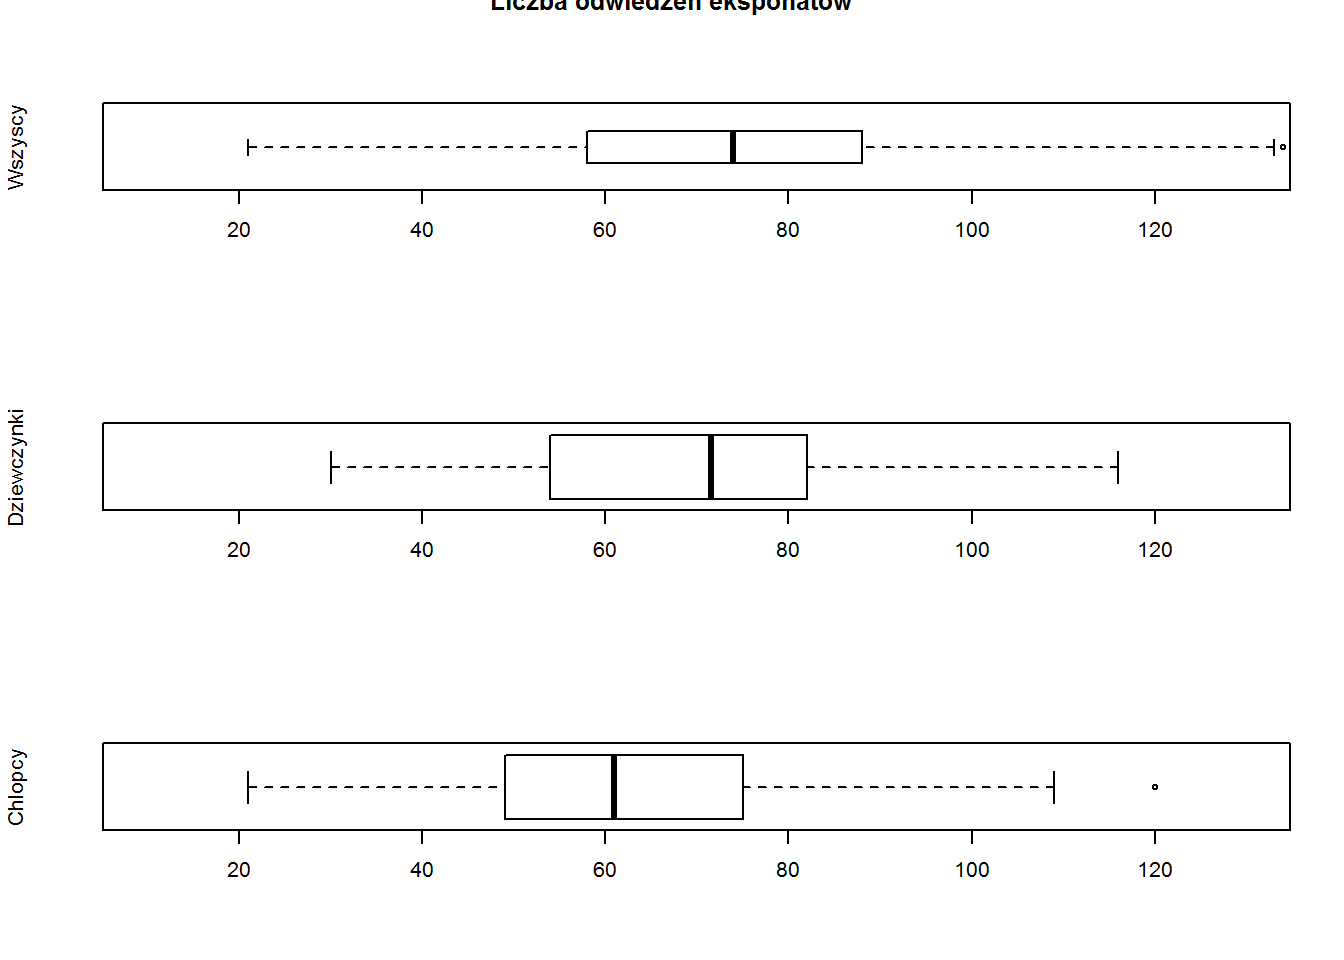
\includegraphics[width=0.48\textwidth]{odwiedziny_plcie.png}
\caption{Liczba odwiedzeń eksponatów w zależności od płci}
\label{odwiedziny_plcie}
\end{figure}
Pierwszy z wykresów przedstawiający odwiedziny wszystkich dzieci zawiera dane o wszystkich dzieciach, a dwa następne jedynie o tych, które wypełniały ankietę -- wskazuje to na istotne braki w danych.

\subsection{Wielokrotne odwiedzanie eksponatów}
Średnia liczba odwiedzeń eksponatu przez dziecko, które już go odwiedziło, wynosi:
\begin{itemize}
\item Dla wszystkich dzieci: 1.228,
\item Dla 20 dzieci z najwyższym kapitałem naukowym: 1.167,
\item Dla 20 dzieci z najniższym kapitałem naukowym: 1.234.
\end{itemize}
Rangowy test Wilcoxona potwierdza, że różnica między dziećmi z najwyższym kapitałem, a pozostałymi, jest statystycznie istotna -- rzadziej podchodzą więcej niż raz do tego samego eksponatu.
\subsection{Liczba unikalnych odwiedzeń eksponatów}
Średnia liczba unikalnych odwiedzeń eksponatów przez dzieci to:
\begin{itemize}
\item Dla wszystkich dzieci: 54.1,
\item Dla 20 dzieci z najwyższym kapitałem naukowym: 55.4,
\item Dla 20 dzieci z najniższym kapitałem naukowym: 49.4.
\end{itemize}
Ponieważ test Shapiro-Wilka nie odrzucił hipotezy o normalności rozkładu tych danych, w celu sprawdzenia statystycznej istotności różnic, zastosowany został t-test Studenta. Na jego podstawie różnice nie są istotne.

\section{Analiza eksponatów}
\subsection{Popularność galerii}
Rysunek \ref{galerie} przedstawia liczbę odwiedzeń eksponatów w poszczególnych galeriach -- w wersji nieprzetworzonej, a także znormalizowanej ze względu na liczbę eksponatów w galerii.
\begin{figure}[H]
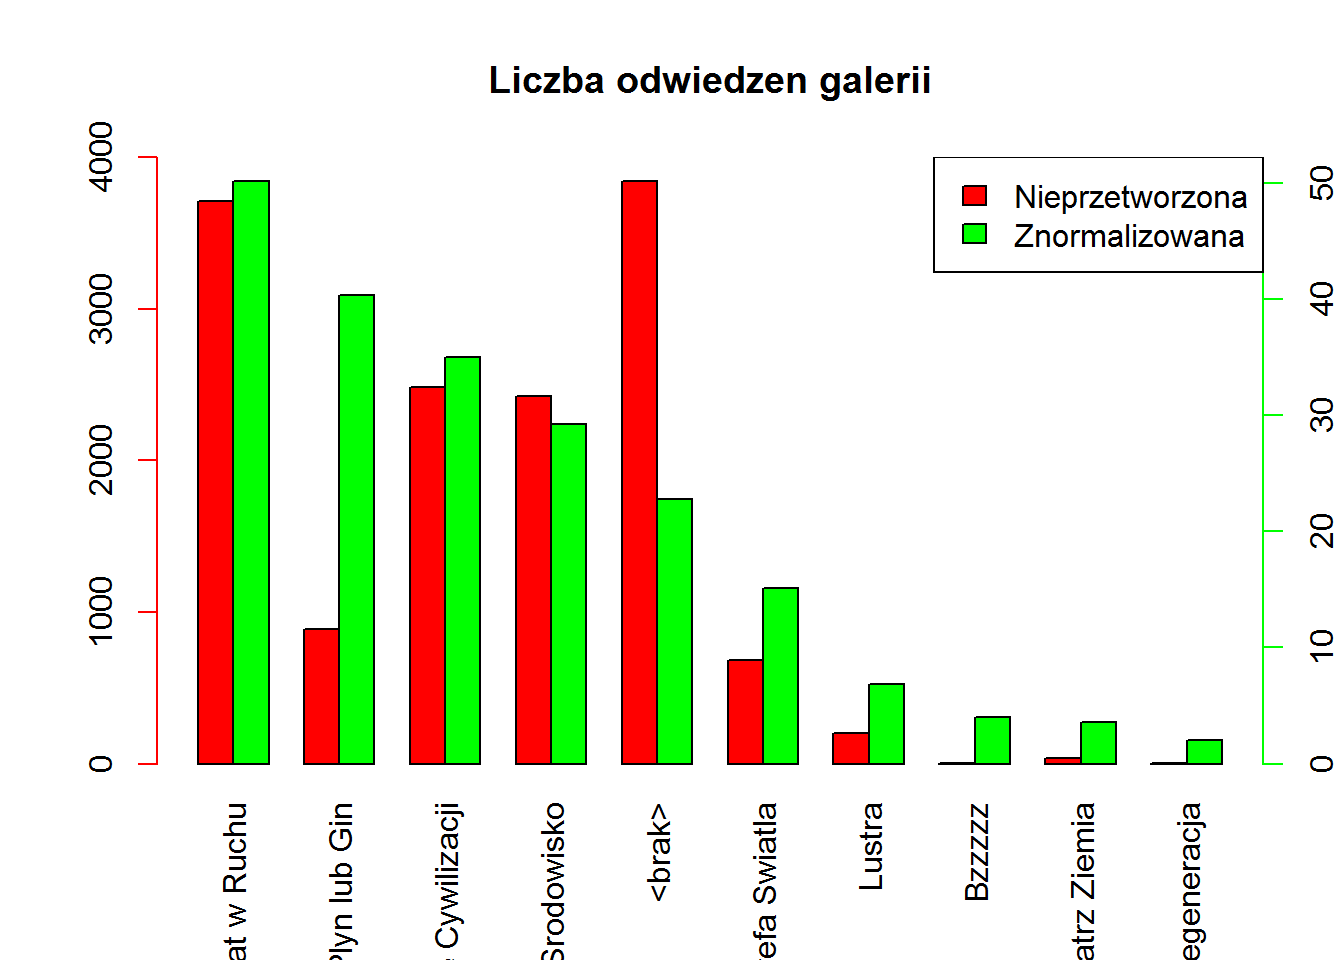
\includegraphics[width=0.48\textwidth]{galerie.png}
\caption{Liczba odwiedzeń poszczególnych galerii}
\label{galerie}
\end{figure}
Normalizacja nie jest w pełni dokładna, ponieważ liczone były jedynie te eksponaty, które zostały odwiedzone co najmniej raz (ze względu na brak kompletnej listy eksponatów) -- anomalie wynikające z tego są szczególnie widoczne w przypadku trzech ostatnich galerii, których liczba odwiedzeń była bardzo niewielka.
\subsection{Popularność eksponatów}
Tabela \ref{top_eksponaty} przedstawia listę najpopularniejszych eksponatów.
\begin{table}[H]
\caption{Najpopularniejsze eksponaty}
\label{top_eksponaty}
\centering
\begin{tabular}{|r|l|l|l|}
\hline
\textbf{Lp.} & \textbf{Eksponat} & \textbf{Galeria} & \textbf{Odwiedziny} \\
\hline
 1 &   ALARM NA STATKU  &     Plyn lub Gin     &         220 \\
 2 &   OKNO KOPERNIKA & Nowy Swiat w Ruchu    &          209 \\
 3 &   MYDLANA SCIANA & Nowy Swiat w Ruchu   &           113 \\
 4 &           CHOMIK  &           ---    &          111 \\
 5 &          TORNADO & Nowy Swiat w Ruchu    &          110 \\
 6 & DOMEK ZE SKRZYNIA  &           ---   &          108 \\
\hline
\end{tabular}
\end{table}
Jak widać, pierwzse dwa eksponaty cieszyły się szczególną popularnością.
\subsection{Najpopularniejsze eksponaty w obrębie każdej galerii}
Tabela \ref{top_eksponaty_galerie} pokazuje najpopularniejszy eksponat w każdej galerii.

\begin{table}[H]
\caption{Najpopularniejsze eksponaty w obrębie każdej galerii}
\label{top_eksponaty_galerie}
\centering
\begin{tabular}{|r|l|l|l|}
\hline
\textbf{Lp.} & \textbf{Galeria} & \textbf{Eksponat} & \textbf{Odw.} \\
\hline

1  &          Plyn lub Gin &           ALARM NA STATKU &  220  \\
2  &    Nowy Swiat w Ruchu &            OKNO KOPERNIKA &              209  \\
3  &                ---    &                    CHOMIK &              111  \\
4  &  Korzenie Cywilizacji &            LASEROWA HARFA &               95  \\
5  & Czlowiek i Srodowisko & BIEGANIE (3,2,1\ldots START!) &               83  \\
6  &        Strefa Swiatla &        UKRYTA PERSPEKTYWA &               42  \\
7  &                Lustra &    ZWIERCIADLANY LABIRYNT &               30  \\
8  &          Patrz Ziemia &     ODBIORNIK SATELITARNY &                7  \\
9  &                Bzzzzz &                  OSWOJAKI &                4  \\
10 &           Regeneracja &      ROZPOZNAWANIE TWARZY &                2  \\
\hline
\end{tabular}
\end{table}
Zgodnie z intuicją, w rzadziej odwiedzanych galeriach (patrz rys. \ref{galerie}) również najpopularniejsze eksponaty otrzymały znacząco mniejszą liczbę odwiedzin.

\subsection{Najbardziej absorbujące eksponaty}
Przeprowadzona została analiza najbardziej absorbujących eksponatów, według następujących kryteriów:
\begin{itemize}
\item Średniego spędzonego czasu,
\item Średniego osiąganego poziomu eksploracji,
\item Frakcji dzieci, które przeczytały opis,
\item Frakcji dzieci, które rozmawiały z animatorem.
\end{itemize}
Dla każdego z tych kryteriów zostały znalezione wiodące eksponaty. Uwzględniane były jedynie eksponaty, które zostały odwiedzone ponad 10 razy, w celu odrzucenia anomalii spowodowanej bardzo małą próbką. Ponadto, znalezione zostały najlepsze według tych kryteriów eksponaty w obrębie każdej galerii, z wyłączeniem trzech najrzadziej odwiedzanych. Dla niektórych kryteriów dodatkowo powstały dodatkowe listy pomijające eksponaty nieposiadające galerii, ze względu na ich widoczną dominację.
\subsubsection{Średni spędzony czas}
Średni czas spędzony na pojedynczym eksponacie to 56.5 sekundy. Tabela \ref{top_czas} przedstawia eksponaty, przy których wizyty średnio zajmowały najwięcej czasu. Podany czas jest reprezentowany w sekundach.

\begin{table}[H]
\caption{Średni czas wizyty przy eksponacie}
\label{top_czas}
\centering
\begin{tabular}{|r|l|l|l|}
\hline
\textbf{Lp.} & \textbf{Eksponat} & \textbf{Galeria} & \textbf{Czas} \\
\hline
1  &         PRZEBUDOWA &                --- &  408.4    \\
2  &       MEMORY FLOOR &                --- &  275.7    \\
3  &             OCULUS &                --- &  256.2    \\
4  &    PIJANY KIEROWCA & Czlowiek i Srodowisko &  181.2    \\
5  &  POJEDYNEK UMYSLOW & Czlowiek i Srodowisko &  179.6    \\
6  & LABIRYNT PRZESZKOD & Czlowiek i Srodowisko &  167.3    \\
7  & KOSMICZNY SMIETNIK &    Nowy Swiat w Ruchu &  162.6    \\
8  &             SEKCJA &                --- &  157.4    \\
9  & AUKCJA HOLENDERSKA &  Korzenie Cywilizacji &  150.6    \\
10 &           ANATOMIA &                --- &  149.4    \\
\hline
\end{tabular}
\end{table}
Pierwsze trzy eksponaty istotnie wyróżniają się. Warto zauważyć, że są to eksponaty poza galeriami. Pozostałe siedem eksponatów ma już bardziej zbliżony średni czas wizyty.

W tabeli \ref{top_czas_g} wskazane są eksponaty o najdłuższym średnim czasie wizyty dla każdej galerii.
\begin{table}[H]
\caption{Średni czas wizyty przy eksponacie}
\label{top_czas_g}
\centering
\begin{tabular}{|r|l|p{3.4cm}|l|}
\hline
\textbf{Lp.} & \textbf{Galeria} & \textbf{Eksponat} & \textbf{Czas} \\
\hline
1 &                ---    &              PRZEBUDOWA    & 408.4 \\
2 & Czlowiek i Srodowisko &            PIJANY KIEROWCA & 181.2 \\
3 &  Korzenie Cywilizacji &         AUKCJA HOLENDERSKA & 150.6 \\
4 &                Lustra &               DUCH PEPPERA & 49.4 \\
5 &    Nowy Swiat w Ruchu &         KOSMICZNY SMIETNIK & 162.6 \\
6 &          Plyn lub Gin & ZJAZD DO TRATWY RATUNKOWEJ & 132.5 \\
7 &        Strefa Swiatla &              ZOLTE SWIATLO & 111.8 \\
\hline
\end{tabular}
\end{table}
Zgodnie z przewidywaniami, istotną grupą wśród najdłużej używanych eksponatów są wystawy w formie gier, tak jak \textit{Kosmiczny śmietnik}, czy \textit{Pijany kierowca}. Poza wcześniej wspomnianymi odstającymi obserwacjami spoza galerii, to zestawienie ujawniło, że eksponaty w galerii \textit{Lustra} są wykorzystywane bardzo krótko -- najdłuższy czas w tej galerii, 49.4 sekundy, to mniej, niż przeciętny czas spędzony przy eksponacie w obrębie całego centrum nauki. 
\subsubsection{Średni osiągnięty poziom eksploracji}
Ponieważ zdecydowaliśmy, że ,,bezmyślne" dotykanie eksponatu nie jest wyższym poziomem, niż patrzenie (a w wielu przypadkach można nawet stwierdzić, że to niższy poziom), pierwotna skala została zmodyfikowana -- 1 oznacza jedynie dotykanie lub jedynie patrzenie, 2 -- korzystanie, a 3 -- eksperymentowanie. Średni poziom w tej skali dla wszystkich eksponatów to 1.66. Warto zwrócić uwagę, że nie wszystkie eksponaty pozwalały na każdy poziom -- na niektóre można było tylko patrzeć, a w wielu nie były możliwe eksperymenty. Tabela \ref{top_zach} przedstawia najbardziej eksplorowane wystawy.
\begin{table}[H]
\caption{Średni poziom eksploracji}
\label{top_zach}
\centering
\begin{tabular}{|r|l|l|l|}
\hline
\textbf{Lp.} & \textbf{Eksponat} & \textbf{Galeria} & \textbf{Poziom} \\
\hline
1  &                DJ &             ---        &     2.08    \\
2  &      DUCH PEPPERA &             Lustra     &        2.00 \\
3  &   KOLOROWE CIENIE &     Strefa Swiatla     &        2.00 \\
4  &       PODUSZKOWCE &             ---        &     2.00    \\
5  &          RURA 900 &             ---        &     1.96    \\
6  &  PRZEWROTNA KULKA & Nowy Swiat w Ruchu     &        1.95 \\
7  &          RUROCIAG &             ---        &     1.95    \\
8  &            MOTORY &             ---        &     1.94    \\
9  &           NA FALI &             ---        &     1.92    \\
10 &          ANATOMIA &             ---        &     1.92    \\
\hline
\end{tabular}
\end{table}
Narzucającą się na pierwszy rzut oka obserwacją jest zdecydowana dominacja eksponatów spoza galerii -- sugeruje to, że zwykle są one bardziej interaktywne, niż pozostałe. Warto też zwrócić na eksponat \textit{Duch Peppera}: jest to eksponat z galerii \textit{Lustra}, przy którym dzieci spędzały najwięcej czasu (a jednocześnie poniżej przeciętnej) -- na podstawie powyższych informacji można wywnioskować, że po prostu ten eksponat nie wymagał dużo czasu, ponieważ trudno by było uwierzyć, żeby z jakiegokolwiek innego powodu dzieci spędzały go tak mało przy wyjątkowo absorbującym eksponacie.
Tabela \ref{top_zach_b} nie uwzględnia eksponatów bez galerii.
\begin{table}[H]
\caption{Średni poziom eksploracji}
\label{top_zach_b}
\centering
\begin{tabular}{|r|l|l|l|}
\hline
\textbf{Lp.} & \textbf{Eksponat} & \textbf{Galeria} & \textbf{Poziom} \\
\hline
1  &       DUCH PEPPERA &                Lustra & 2.00 \\
2  &    KOLOROWE CIENIE &        Strefa Swiatla & 2.00 \\
3  &   PRZEWROTNA KULKA &    Nowy Swiat w Ruchu & 1.95 \\
4  &     ORKIESTRA TUSZ &  Korzenie Cywilizacji & 1.89 \\
5  &        ZYWE SREBRO &    Nowy Swiat w Ruchu & 1.89 \\
6  &              DIETA & Czlowiek i Srodowisko & 1.88 \\
7  &   WAHADLO SWIETLNE &    Nowy Swiat w Ruchu & 1.88 \\
8  & MAGNETYCZNA CHMURA &    Nowy Swiat w Ruchu & 1.86 \\
9  &       WYSCIG LODZI &  Korzenie Cywilizacji & 1.82 \\
10 &      PRZESLUCHANIE &        Strefa Swiatla & 1.81 \\
\hline
\end{tabular}
\end{table}
W tym zestawieniu rozkład galerii jest znacznie bardziej równomierny.
Tabela \ref{top_zach_g} to zestawienie najbardziej eksplorowanych eksponatów w obrębie każdej galerii.

\begin{table}[H]
\caption{Średni poziom eksploracji}
\label{top_zach_g}
\centering
\begin{tabular}{|r|l|l|l|}
\hline
\textbf{Lp.} & \textbf{Galeria} & \textbf{Eksponat} & \textbf{Poziom} \\
\hline
1 &                ---    &            DJ    &  2.08	\\
2 & Czlowiek i Srodowisko &            DIETA &     1.88	\\
3 &  Korzenie Cywilizacji &   ORKIESTRA TUSZ &     1.89	\\
4 &                Lustra &     DUCH PEPPERA &                    2.00	\\
5 &    Nowy Swiat w Ruchu & PRZEWROTNA KULKA &     1.95	\\
6 &          Plyn lub Gin &   SRUBA NAPEDOWA &     1.56	\\
7 &        Strefa Swiatla &  KOLOROWE CIENIE &                    2.00	\\
\hline
\end{tabular}
\end{table}
W powyższym zestawieniu warto zwrócić uwagę, że najbardziej eksplorowana wystawa z galerii \textit{Płyń lub giń} ma poziom 1.56, czyli niższy, niż średni w obrębie całej galerii -- można wnioskować, że to w tej galerii dzieci najczęściej bezmyślnie się bawią lub tylko obserwują. 

\subsubsection{Frakcja dzieci, które przeczytały opis}
Opis był czytany przez dzieci w 10\% przypadków. Należy zauważyć, że przeczytanie opisu raczej nie implikuje, że eksponat jest ciekawszy niż inne -- dzieci najprawdopodobniej robią to w ostateczności, jeśli bez tego nie mogą zrozumieć eksponatu. Z drugiej strony, jeśli wystawa nie wydaje im się ciekawa i jej nie rozumieją, dużo dzieci zamiast przeczytania opisu może się zniechęcić i odejść -- tak więc możliwym jest, że eksponaty, przy których dzieci najczęściej czytały opis, były relatywnie skomplikowane, ale jednocześnie ciekawe.
Tabela \ref{top_opis} przedstawia wystawy, przy których dzieci najczęściej sięgały po opis.
\begin{table}[H]
\caption{Frakcja dzieci, które przeczytały opis}
\label{top_opis}
\centering
\begin{tabular}{|r|p{3.3cm}|l|l|}
\hline
\textbf{Lp.} & \textbf{Eksponat} & \textbf{Galeria} & \textbf{Opis} \\
\hline
1  &                  DUCH PEPPERA &                Lustra & 0.58 \\
2  &                 RADIO W GEBIE &    Nowy Swiat w Ruchu & 0.39 \\
3  &              FIGURY LISSAJOUS &    Nowy Swiat w Ruchu & 0.36 \\
4  &             OCZY Z TYLU GLOWY &                Lustra & 0.36 \\
5  & CZESCI ZAMIENNE DLA CZLOWIEKA & Czlowiek i Srodowisko & 0.36 \\
6  &                  PALACY CHLOD & Czlowiek i Srodowisko & 0.35 \\
7  &               CHCA BYC PIEKNI & Czlowiek i Srodowisko & 0.33 \\
8  &        PO GLOSIE CIE POZNAJA? & Czlowiek i Srodowisko & 0.33 \\
9  &       PRZENOSNY MOST LEONARDA &  Korzenie Cywilizacji & 0.33 \\
10 &                SKACZACA KULKA &    Nowy Swiat w Ruchu & 0.33 \\
\hline
\end{tabular}
\end{table}
Tylko przy jednej wystawie ponad połowa zwiedzających dzieci przeczytała opis. Wystąpiły aż dwa eksponaty z galerii \textit{Lustra} (w której było niewiele odwiedzonych eksponatów), w której maksymalny czas był mniejszy, niż średni czas z całego centrum nauki -- potwierdza to tezę, że wcześniejsza obserwacja wynikała jedynie z charakteru eksponatów, a nie braku zainteresowania. Ponadto, w zestawieniu nie wystąpił ani jeden eksponat bez galerii.
Tabela \ref{top_opis_g} to zestawienie eksponatów, które najczęściej wymagały czytania opisu, dla każdej galerii.
\begin{table}[H]
\caption{Frakcja dzieci, które przeczytały opis}
\label{top_opis_g}
\centering
\begin{tabular}{|r|l|p{3.3cm}|l|}
\hline
\textbf{Lp.} & \textbf{Galeria} & \textbf{Eksponat} & \textbf{Opis} \\
\hline
1 &                ---    &              OCZYSZCZALNIA    & 0.29 \\
2 & Czlowiek i Srodowisko & CZESCI ZAMIENNE DLA CZLOWIEKA & 0.36 \\
3 &  Korzenie Cywilizacji &       PRZENOSNY MOST LEONARDA & 0.33 \\
4 &                Lustra &                  DUCH PEPPERA & 0.58 \\
5 &    Nowy Swiat w Ruchu &                 RADIO W GEBIE & 0.39 \\
6 &          Plyn lub Gin &                 LODZ PODWODNA & 0.23 \\
7 &        Strefa Swiatla &               ZIELONY PROMIEN & 0.29 \\
\hline
\end{tabular}
\end{table}
W przypadku czytania opisu, znacząco wyróżnia się tylko galeria \textit{Lustra}.

\subsubsection{Frakcja dzieci, które rozmawiały z animatorem}
Tylko 4\% wizyt wiązało się z rozmową z animatorem. Tabela \ref{top_animator} pokazuje eksponaty, przy których najczęściej dochodziło do takiej interakcji.
\begin{table}[H]
\caption{Frakcja dzieci, które rozmawiały z animatorem}
\label{top_animator}
\centering
\begin{tabular}{|r|p{3cm}|l|l|}
\hline
\textbf{Lp.} & \textbf{Eksponat} & \textbf{Galeria} & \textbf{Rozmowa} \\
\hline
1  &                ANATOMIA &               --- & 0.67 \\
2  &         WYSTAWA CZASOWA &               --- & 0.43 \\
3  &       LEWITUJACY BACZEK &   Nowy Swiat w Ruchu & 0.42 \\
4  & PRZENOSNY MOST~LEONARDA & Korzenie Cywilizacji & 0.33 \\
5  &                  SEKCJA &               --- & 0.33 \\
6  &                MROZENIE &               --- & 0.29 \\
7  &                    PULS &               --- & 0.28 \\
8  &            ZAGRYZ NUTKE &               --- & 0.28 \\
9  &                   HANOI & Korzenie Cywilizacji & 0.25 \\
10 &                 KRZESLA &               --- & 0.25 \\
\hline
\end{tabular}
\end{table}
Prawie wszystkie z wiodących obserwacji nie należą do żadnej galerii -- wyjaśnia to, dlaczego dla eksponatów spoza galerii dzieci rzadko czytały opis.

Tabela \ref{top_animator_b} to zestawienie z wykluczeniem wystaw bez galerii.
\begin{table}[H]
\caption{Frakcja dzieci, które rozmawiały z animatorem}
\label{top_animator_b}
\centering
\begin{tabular}{|r|p{3cm}|l|l|}
\hline
\textbf{Lp.} & \textbf{Eksponat} & \textbf{Galeria} & \textbf{Rozmowa} \\
\hline
1  &       LEWITUJACY BACZEK &    Nowy Swiat w Ruchu & 0.42 \\
2  & PRZENOSNY MOST~LEONARDA &  Korzenie Cywilizacji & 0.33 \\
3  &                   HANOI &  Korzenie Cywilizacji & 0.25 \\
4  &           ZOLTE SWIATLO &        Strefa Swiatla & 0.25 \\
5  &      CZLOWIEK UKLADANKA & Czlowiek i Srodowisko & 0.24 \\
6  &             WYCIERACZKI &        Strefa Swiatla & 0.23 \\
7  &         ZAPISY LICZBOWE &  Korzenie Cywilizacji & 0.18 \\
8  &      ROWEROWE PRZEKRETY &    Nowy Swiat w Ruchu & 0.18 \\
9  &               ZALADUNEK &          Plyn lub Gin & 0.17 \\
10 &                   DIETA & Czlowiek i Srodowisko & 0.15 \\
\hline
\end{tabular}
\end{table}
Otrzymane wyniki znacznie przewyższają średnią -- przypuszczalnie przy niektórych eksponatach animatorzy byli znacznie częściej, niż przy innych.

W tabeli \ref{top_animator_g} przedstawione są eksponaty w obrębie galerii, dla których najczęściej dochodziło do rozmowy z animatorem.
\begin{table}[H]
\caption{Frakcja dzieci, które rozmawiały z animatorem}
\label{top_animator_g}
\centering
\begin{tabular}{|r|l|p{3cm}|l|}
\hline
\textbf{Lp.} & \textbf{Galeria} & \textbf{Eksponat} & \textbf{Rozmowa} \\
\hline
1 &                --- &                ANATOMIA &  0.67	\\
2 & Czlowiek i Srodowisko &      CZLOWIEK UKLADANKA &  0.24	\\
3 &  Korzenie Cywilizacji & PRZENOSNY MOST~LEONARDA &  0.33	\\
4 &                Lustra &  ZWIERCIADLANY LABIRYNT & 0.03	\\
5 &    Nowy Swiat w Ruchu &       LEWITUJACY BACZEK &  0.42	\\
6 &          Plyn lub Gin &               ZALADUNEK &  0.17	\\
7 &        Strefa Swiatla &           ZOLTE SWIATLO &  0.25 \\
\hline
\end{tabular}
\end{table}
Widoczną anomalią jest galeria \textit{Lustra}, dla której maksymalnie tylko 3\% odwiedzeń wiązało się z rozmową z animatorem, co jest mniejszą wartością, niż średnia z Centrum Nauki Kopernik. Przypuszczalnie wiąże się to ze specyfiką galerii (eksponaty, przez które szybko się przechodzi), a jednocześnie tłumaczy to częstsze sięganie przez dzieci po opis.

\section{Wnioski}








\end{document}


